\subsection{Game}
I "Game" klassen er der hvor spillet kører (while loop). Loopet kører indtil der er blevet fundet en vinder udfra "Logic" klassens vinde betingelse. 
\begin{figure}[H]
    \centering
    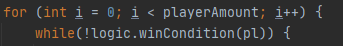
\includegraphics{sources/7_implementering/gameLoop.PNG}
    \caption{"While loop" indtil en vinder er fundet}
    \label{fig:mainLoop}
\end{figure}

Det er også at Chancekort bliver trukket til spillerne fra chancekort dækket(klassen).

\begin{figure}[H]
    \centering
    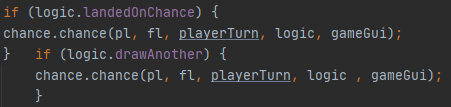
\includegraphics{sources/7_implementering/gameChance.PNG}
    \caption{Hvis spilleren er landet på et chancefelt træk da et chancekort}
    \label{fig:chance}
\end{figure}
